\documentclass[12pt]{article}

%%%%%%%%%%%%%%%%%%%%%%%%%%%%%%%%%%%%%% PACKAGES %%%%%%%%%%%%%%%%%%%%%%%%%%%%%%%%
\usepackage[swedish]{babel}
\usepackage{hyperref}
\usepackage{pgfgantt} % Gantt charts. docs: https://ftpmirror1.infania.net/mirror/CTAN/graphics/pgf/contrib/pgfgantt/pgfgantt.pdf
\usepackage{pdflscape} % Landscape mode

% TODO remove these packages for final report
%%%%%%%%%%%%%%%%%%%%%%%%%%%%%%%% "Debug" packages %%%%%%%%%%%%%%%%%%%%%%%%%%%%%%

% Comments in the margin, use \todo{} to add comment to margin.
% Docs: http://tug.ctan.org/macros/latex/contrib/todonotes/todonotes.pdf
\usepackage[colorinlistoftodos]{todonotes}

%%%%%%%%%%%%%%%%%%%%%%%%%%%%%%%%%  TITLE PAGE  %%%%%%%%%%%%%%%%%%%%%%%%%%%%%%%%%

\title{Projektrapport - Dekompilering med ungefärlig symbolisk exekvering}
\author{
    Albin Otterhäll\thanks{GU-IT} \and
    Clara Salber\thanks{GU-IT} \and
    Enayatullah Norozi\thanks{TKDAT} \and
    Linus Wallman\thanks{TKITE} \and
    Loke Gustafsson\thanks{TKTEM} \and
    Samuel Kyletoft\footnotemark[3]
}

%%%%%%%%%%%%%%%%%%%%%%%%%%%%% DOCUMENT STRUCTURE %%%%%%%%%%%%%%%%%%%%%%%%%%%%%%%

\begin{document}
\maketitle

\newpage

% TODO remove this for final report
\listoftodos
\newpage

\tableofcontents
\newpage

Vad repporten ska innehålla:
\url{https://chalmers.instructure.com/courses/22323/assignments/66457?module_item_id=337856}.

\section{Bakgrund}
% BAKGRUNDENS UPPGIFT?: Motivera behovet att visualiseringsverktyg för fuzzing
% (fuzzing används slarvigt, inkludera tex concolic testing)

Att läsa källkod är ett sätt att förstå program, men ibland är det gynnsamt att istället betrakta
maskinkoden direkt. Detta kan vara för att
\begin{itemize}
  \item utesluta påverkan av kompilatorbuggar som ger oväntad maskinkod
  \item se hur undefined behavior (UB) har utnyttjats av kompilatorn
  \item källkoden inte är tillgänglig
\end{itemize}

Det finns en uppsjö av metoder som kan användas för att analysera en exekverbar
binär. Exempel på dessa är:
\todo{källhänvisa}
\begin{enumerate}
  \item disassemblera binären och läsa dess funktioner för att förstå vad de gör.
  \item dekompilera assemblykoden med ett verktyg som ger högnivåpseudokod, och som sedan blir läsbara.
  \item köra binären på speciella testfall och jämföra svaret med vad som förväntas. Om
    programmet implementerar en specifikation kan det istället använda en existerande testsamling.
  \item fuzztesta binären, det vill säga automatiskt generera testfall tills ett orsakar en crash eller
    odefinierat beteende i binären. Många fuzztestmotorer skapar testfall med en evolutionär
    algoritm, och många använder instrumentering över vilka programhopp som tas för att bedöma
    testfalls nyttighet.
  \item använda concolic testing, alltså fuzzing där en SMT solver genererar nya testfall genom att
    lösa för testfall som orsakar annorlunda programhopp.
  \item stega igenom programmet i en debugger för att se exakt vad programmet gör med viss input.
\end{enumerate}

För att bilda en allmän förståelse om programmet krävs både \textit{korrekt} och \textit{abstrakt} förståelse. 
I detta avseende syftar \textit{korrekt} på saknandet av felaktiga slutsatser
och \textit{abstrakt} på möjligheten att resonera om programmet generellt i
motsats till att resonera om specifik konkret indata i taget.

Metod 1-2, att läsa kod, kan ge en \textit{abstrakt} förståelse av vad programmet gör, men för
att verifiera att huruvida resonemanget är korrekt krävs hypotestestning vilket
kräver att programmet körs. Således går det inte att bilda en \textit{korrekt} förståelse genom 
att enbart läsa kod.

Metod 3-5, att köra programmet på testfall, ger framförallt en black-box-förståelse av
programmet. Tillgången till binären och exekveringsmiljön används endast som ett verktyg
för att generera nya testfall. Fuzzing och concolic testing kan köras helautomatiskt och är
\textit{korrekta}. Men ofta är en tillräckligt täckande sökning av indatarummet omöjlig, och då kan
den automatiska analysen ha missat ett kvalitativt annorlunda beteende. Dessutom ger en omfattande
uppsättning indata-utdata-par inte användaren samma information som källkoden ger. Därmed är
helautomatiska analysmetoder inte \textit{abstrakta}. Notera att det inte nödvändigtvis tyder på en
brist i den automatiska analysen att ett kvalitativt annorlunda beteende missas, för det gömda
beteendet skulle kunna vara en konsekvens av komplicerad kod, som till exempel ett hoppvilkor
beroende på en kryptografisk hash av indatan. Men en analysmetod borde kunna peka ut var dess
förståelse tar slut, snarare än att utelämna detta fullständigt vilket är vad avsaknaden av testfall
visar sig som.

Med metod 6, i en debugger, kan användaren följa exekveringen för en viss indata utan att riskera
att missförstå hur datan transformeras. Om användaren har ett oändligt tålamod kan de göra detta om
och om igen för olika indata genererade med till exempel fuzzing. Varje genomstegning ger
information om koden som behandlar indatan men också viss information om övrig kod -- till exempel
kan ett svårtaget hopp indikera en plats för användaren att rikta sin uppmärksamhet mot. Detta ger
en både \textit{korrekt} och \textit{abstrakt} förståelse, men med en orimlig manuell arbetsbörda
för användaren.

En helautomatisk \textit{korrekt} metod kan ge en \textit{abstrakt} förståelse om processens förlopp
visualiseras för användaren. Valet mellan manuell arbetsbörda som ger djup förståelse och en
testfallsgenerationsdriven process som ger översiktlig förståelse kan genomföras av användaren om
verktygen stödjer hela spektrat.


\section{Syfte}
Projektets mål är att utveckla ett binäranalysverktyg som möjliggör effektivt
analys av binära program utan tillgång till källkoden. Fokuset ligger på
användbara analysfunktioner som hoppas kunna kombineras med intuitiv
användargränssnitt för att vara tilltalande till en mångsidig målgrupp,
inklusive säkerhetsforskare och programvaruutvecklare. Vektyget är tänkt att
bidra till ökad hantering av säkerhetsaspekterna i tekniska system.


\section{Problem/Uppgift}
% Det här avsnittet är ofta den viktigaste delen av planeringsrapporten (och av
% den slutgiltiga uppsatsen/rapporten). Den syftar till att identifiera
% frågan/frågorna som ska tas upp i projektet. Det är viktigt att gruppen gör en
% problemanalys även om det i projektförslaget redan finns ett problem (en
% uppgift) specificerat. Anledningen till detta är att det riktiga primära
% problemet ofta skiljer sig från det i början av
% uppdragsgivaren/förslagsställaren/kunden föreslagna. Problemanalysen syftar
% också till att bryta ner problemet/uppgiften i mindre och mer detaljerade
% delproblem/deluppgifter, vilket också leder till formulering av delsyften.
% Genom att göra detta får studenterna mycket bättre förståelse för de olika
% aspekterna av problemet/uppgiften. Utan den här informationen är det omöjligt
% att identifiera vilken information som behövs, vilka informationskällor som
% behövs och lämpliga tillvägagångssätt.

% En bra problemanalys som identifierar delproblem/deluppgifter och delsyften
% vilar i många fall på användning av teorier och modeller från litteraturen. En
% litteraturgenomgång bör därför genomföras tidigt i processen.

För att uppnå projektets syfte om att konstruera ett symboliskt-kapabelt
binäranalysverktyg delas denna uppgift upp i mindre delar.

Kärnan i ett \textit{korrekt} binäranalysverktyg är en
\textit{exekveringsmotor}, en komponent som på ett korrekt vis kan köra
programmet. Att köra ett program innebär att ladda binären och dess bibliotek,
hoppa till startadressen och sedan köra enskilda instruktioner. Om
binäranalysverktyget ska kunna använda metoder som använder symbolisk exekvering
behöver denna exekvering av enskilda instruktioner också stödja symboliska
variabler. För att verktyget ska uppnå hög prestanda är det eftersträvansvärt
att de instruktioner som inte använder symboliska variabler utan endast agerar
på konkreta värden exekverar direkt på processorn som kör binäranalysverktyget.

Program i verkligheten kommunicerar på många sätt med sin omgivning. För
inbyggda system är denna omgivning fysisk och för program som kör ovanpå
operativsystem är denna omgivning en virtuell värld bestående av filer och inter
process communication (IPC). För att en \textit{exekveringsmotor} ska vara så
brett tillämpbar som möjligt behöver den också stödja flera sorters
omgivningskommunikation.

Sammantaget är kraven på en \textit{exekveringsmotor} med stöd för symbolisk
analys att den \begin{enumerate} \item kan ladda en binär i en konkret miljö
		\item kan introducera symboliska variabler i denna miljö genom till
			exempel omgivningskommunikation \item kan exekvera konkreta delar av
			programmet med god prestanda genom att köra dessa delar av
		programmet som maskinkod \item kan exekvera symboliska delar av
			programmet på ett sätt som är tillräckligt kraftfullt för de
			symboliska analyser som exekveringsmotorn ska användas till
\end{enumerate} Dessutom behöver exekveringsmotorn kunna kontrolleras och dess
slutsatser kunna användas av och presenteras i resten av programmet.
Figur~\ref{schematic} visar förhållandet mellan användaren, analysverktyget och
dess exekveringsmotor.

\begin{figure}[H] \centering 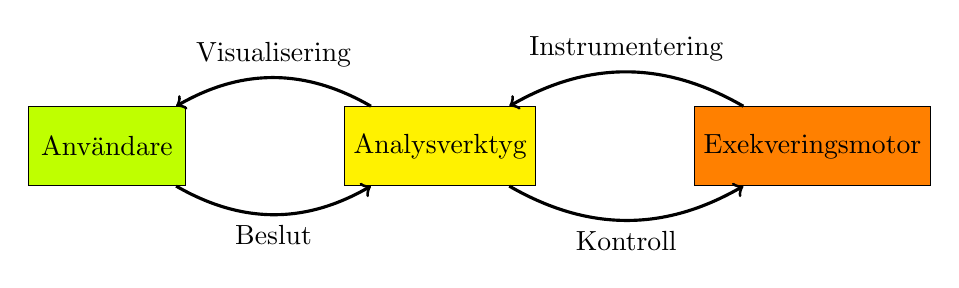
\begin{tikzpicture} \node [draw, fill=lime, minimum
	width=2cm, minimum height=1cm, ]  (user) {Användare};

		\node [draw, fill=yellow, minimum width=2cm, minimum height=1cm,
		right=2cm of user ] (tool) {Analysverktyg};

		\node [draw, fill=orange, minimum width=2cm, minimum height=1cm,
		right=2cm of tool ] (engine) {Exekveringsmotor};

		\draw[->, line width=.4mm] (user.-30) to[out=-30, in=-150]
		node[midway,below]{Beslut} (tool.-150);

		\draw[->, line width=.4mm] (tool.150) to[out=150, in=30]
		node[midway,above]{Visualisering} (user.30);

		\draw[->, line width=.4mm] (tool.-30) to[out=-30, in=-150]
		node[midway,below]{Kontroll} (engine.-150);

		\draw[->, line width=.4mm] (engine.150) to[out=150, in=30]
		node[midway,above]{Instrumentering} (tool.30);

	\end{tikzpicture} \caption{ Schematisk bild av ett binäranalysverktyg byggt
	kring en exekveringsmotor }\label{schematic} \end{figure}

\subsection{Analyser}

Det finns många möjliga analyser som kan användas av ett binäranalysverktyg, där
\textit{analyser} avser en visualisering av en aspekt av det analyserade
programmets beteende eventuellt inklusive ett sätt för användaren att påverka
det analyserade programmets körning.

En konkret exekvering kan spåras och dess instruktionssekvens kan visas för
användaren med loopar identifierade. Flera exekveringar kan visualiseras på
samma sätt och deras instruktionssekvenser användas för att återskapa
kontrollflödesstrukturer som for- och while-loopar och if-satser.

Möjligheter för \textit{state merging} kan identifieras helautomatiskt eller av
användaren, alltså platser där flera exekveringar kan ersättas av en enda mer
generell exekvering som innehåller ursprungsexekveringarnas skillnader som
symboliska uttryck.

En uppsättning liknande exekveringar kan visas upp för användaren tillsammans
med information om när och hur de divergerar, för att till exempel avgöra när
olika delar av indatan används.

För analys av programmet är det också hjälpsamt för användaren att kunna stega
genom exekveringen steg för steg och ändra på värden för att ta de vägar de vill
analysera. Detta borde också kunna göras baklänges, det vill säga att användaren
väljer en slutdestination och låter programmet själv lista ut vilka värden som
behövdes läsas för att exekveringen skulle ta sig till den punkten.

En mer automatisk men ändå viktig funktionalitet är konstruktion av kod-täckande
indata. När testfall som besöker en uppsättning instruktioner är konstruerad kan
kraven på indatan över denna uppsättning programhopp analyseras och programmet
kan lista ut vilka aspekter av indatan som kan ändras utan att påverka
kodtäckningsgraden, och kommunicera detta till användaren.

Det finns många möjliga analyser. Användbarheten i ett verktyg mäts inte i
kvantiteten analyser utan i förmågan för de utvalda implementerade analyserna
att täcka användarens behov av förståelse av programmet.


\section{Avgränsningar}

%motivera s2e:
% fördel, slipper göra
% specifikt behöver inte tvivla
% svårt att göra en emulator korrekt, vältestat, litar på korrekthet, gör ens jobb mycket enklare


% vad gör s2e och symqemu
% nackdelar med symQemu, docs saknas

% detaljerat men inte långt

% S²E comes as a modular library that gives virtual machines symbolic execution and program analysis
% capabilities. S²E runs unmodified x86, x86-64, or ARM software stacks, including programs, libraries,
% the kernel, and drivers. Symbolic execution then automatically explores hundreds of thousands of paths
% through the system, while analyzers check that the desired properties hold on these paths and selectors
% focus path exploration on components of interest.
% SymQemu has not been actively maintained in recent years and it may not be compatible with the latest
% versions of QEMU and KLEE. It is recommended to use more modern tools for dynamic analysis, such as S2E,
% which provide similar capabilities with a more up-to-date infrastructure.


Att skapa en emulator är tidskrävande, dessutom är den resulterande produktens
korrekthet inte tillförlitlig utan nogrann testning. För att fastställa
korrekthet premieras därför att använda ett existerande verktyg för att
exekvera programmet med stöd för symbolisk exekvering. Detta möjliggör också
bredade plattformssupport jämfört med en hemmasnickrad emulator.

\subsection{S2E}

\todo{skriva om S2E}

\subsection{SymQEMU}

\todo{skriva om SymQEMU}

\subsection{Beslut}

\todo{motivera S2E}

Applikationen ska utvecklas med hjälp av S2E, som bygger ut QEMU:s virtuella
maskin med stöd för symbolisk exekvering. S2E är i sin tur utbyggbart med möjlighet
för användaren att skriva egna plugins för att utföra analyser och används
bland annat inom flygindustrin, forskning och cybersäkerhet. Detta i
kombination med att S2E är open-source och aktivt underhållet gör S2E till
ett passande verktyg för vår applikation.

Ett alternativt verktyg för symbolisk exekvering är symQEMU, som kombinerar
QEMUs virtuella maskin med KLEEs motor för symbolisk exekvering. Då SymQEMU
ej uppdateras aktivt och har bristfällig dokumentation föredrogs S2E.

Projektet avgränsas i och med att existerande verktyg (S2E) kommer användas
istället för att bygga en motor för symbolisk exekvering från grunden. Att
använda S2E innebär att arbetet avgränsas till att skapa ett plugin som bygger
ut motorn. Varken emulator eller motor ska byggas och de uppgifter som ingår i
att skapa en dekompilator exkluderas.

\subsection{Konsekvenser}

Beslutet innebär att applikationens utformning blir bunden till verktygens
tekniska begränsningar.

Avgränsningen medför dessutom att fokus flyttas ifrån motorns tekniska detaljer
till att utveckla en användbar slutprodukt som bygger ut S2E's redan
existerande funktionalitet med ett grafiskt användargränsnitt och möjlighet att
stega igenom, analysera och interaktivt besluta om värden under exekvering.


\section{Metod/Genomförande}
\subsection{Val av strategi}
För att uppnå och redogöra för möjligheterna i en potentiell applikation reflekterades det över två möjliga 
alternativ att fullfölja. Dels diskuterades alternativet att bygga en symbolic execution engine från grunden och fokusera på
dess tekniska detaljer och dels att använda en existerande produkt där fokuset istället ligger på att bygga plugins vars
syfte är att utöka den existerande motorn med fler funktioner. 

Med syfte att göra framsteg valdes det att kolla vidare hur SymQEMU kan hjälpa i frågan om att utöka funktionalitet
i en existerande motor. SymQEMU är utvecklat i största del C/C++ och med anledning av valet att utveckla i ett annat
programmeringsspråk, det vill säga Rust, krävs implementation C/C++-bindings. I ett första steg valdes därför att 
se över hur detta går till på lämpligast sätt och hur detta kan automatiseras med hjälp av andra verktyg där bland annat 
autocxx ansågs som ett lovande alternativ. 

\subsection{Tillvägagångssätt}





\section{Samhälleliga och etiska aspekter, bedömning om det behöver beaktas för vald problemställning}
% Lärandemål i kursplanen för kandidatarbetet:
% "bedöma om samhälliga och etiska aspekter behöver beaktas för vald problemställning och där det är relevant, analysera dessa aspekter i uppsatsen/rapporten

% Beslutsmodell för kritiskt tänkande om etiska frågor
% Denna modell är tänkt att användas så att gruppen går igenom frågorna en gång och svara på dem preliminärt.
% När gruppen gjort detta kan de gå igenom frågorna igen för att fördjupa analysen.

När vi skriver \emph{försvarare} syftar vi på de personer som har till uppgift att upprätthålla  ett datorsystems konfidentialitet; tillgänglighet; och integritet.
Med \emph{attackerare} syftar vi på de personerna som har som mål att negativt påverka ett datorsystems konfidentialitet; tillgänglighet; eller integritet.

\subsection{Q1: Vilka etiska aspekter (värden) är relevanta för projektet?}

% Det finns några få centrala etiska aspekter vilka alltid är viktiga att undersöka om de är relevanta – och om så är fallet – uppfylla dessa.
% Dessa är att vi inte ska göra skada, vi ska göra nytta, och vi ska inte inskränka på andras autonomi och integritet.
% Att göra nytta ska här tolkas brett: både den inomvetenskapliga och utomvetenskapliga nyttan är relevant.
% Till exempel kan det vara så att ett projekt inte har någon specifik nytta för samhället men att det ändå finns goda skäl att genomföra det eftersom det skulle tillföra något intressant och relevant till grundforskningen.
% Beroende på projektet kan det finnas andra relevanta aspekter att ta hänsyn till.

En stor del av teknikutveckling av verktyg som har som mål att hjälpa försvarare med att hitta säkerhetsbrister i deras programvarar kan även användas av attackerare.
Medan försvararna använder verktygen för att hitta brister för att de ska veta vilka åtgärder de ska vidta för att höja säkerheten, använder attackerarna verktygen för att hitta brister som de sedan kan uttnytja för att påverka datorsystem negativt.
Alltså använder försvarare och attackerna verktygen på liknande sätt, men vad de sedan gör med den informationen skiljer dem åt.

- Ökad förståelse för hur program exekverar. Det gör det möjligt att hitta buggar i program, eller optimera dem.

Ett möjligt problem är att verktygen som utvecklas för försvararna blir såpass bra att attackerarna helt börjar använda dem för att utföra attacker.

\subsection{Q2: Hur kann vi genomföra vårt projekt för att undvika etiska problem med vår metod?}

% Givet att gruppen ska genomföra ett visst projekt kan det finnas en rad olika sätt som det
% kan utföras på där vissa genomföranden är mer problematiska än andra.
% Ett exempel är ett projekt där studenternas frågeställningar kan undersökas med djurförsök.
% Här bör diskuteras om djurförsöken kan ersättas med andra typer av försök, alternativt använda färre djur, göra
% försöken mindre plågsamma och så vidare.
% Ett annat exempel är ett projekt har som mål att utveckla en teknisk lösning för att minska människors ångestproblematik.
% Studenterna har tänkt testa denna lösning på sina vänner och bekanta.
% I ett sådant projekt är det viktigt att vara medveten om och diskutera att metoden kan medföra problem för deltagarnas välbefinnande.

\subsection{Q3: Vad kan det finnas för nytta eller etiska problem med det sannolika resultatet (utfallet) av projektet som man bör ta hänsyn till?}

% När projektet är genomfört kan det bidra med nytta till både forskning och samhälle.
% Det är viktigt att beskriva nyttan i konkreta termer och också beskriva om projektets färdigställande riskerar att leda till skador på olika sätt.
% Ett exempel är ett projekt som genomförs i en stadsdel med målet att öka tryggheten och delaktigheten för de boende genom en boendedriven innovation, där man bör fundera över vad som troligt händer efter det att projektet avslutas.

\subsection{Q4. Vilka berörs av projektets genomförande eller av det sannolika resultatet (utfallet) av projektet? Hur berörs de? Finns det etiska problem kopplat till detta som man bör ta hänsyn till?}

% Vid en etisk analys av ett projekt är det av yttersta vikt att fråga sig vilka som berörs av projektet samt på vilket sätt de påverkas.
% Till exempel, om ett projekt syftar till att genmodifiera grödor så att de blir mer resistenta mot bekämpningsmedel så kan en effekt av detta bli när dessa grödor kommer ut på marknaden att de bönder som arbetar med dessa grödor i fattigare delar av världen tar stor (ekonomisk och/eller fysisk) skada av detta.
% Eftersom skador på redan utsatta grupper kan bli extra allvarliga från ett etiskt perspektiv, bör denna sorts överväganden få stor vikt.

\subsection{Q5. Vad bör vi göra om vi inte hittat några relevanta etiska aspekter (värden) rörande projektet?}

% Om studentgruppen har gått igenom steg 1-4 ovan och analyserat sitt projekt och projektets möjliga effekter utan att hitta några relevanta etiska eller samhälleliga aspekter byter gruppen analysnivå (systemnivå).
% Beroende på vilken nivå projektet analyseras på kan den utom- och inomvetenskapliga relevansen bedömas på olika sätt.
% Till exempel, gruppens projekt är att i slutändan bidra med att tillsätta en extra skalärboson till standardmodellen.
% Gruppens projekt i sig aktiverar antagligen inte några relevanta etiska aspekter i sitt genomförande eller i sitt utfall.
% Ändå går det att tänka sig att resultaten i det större forskningssammanhanget, som studenternas projekt bidrar till, kan ha en rad olika positiva och negativa implikationer för både forskning och samhälle.
% Ett annat exempel kan vara ett projekt med syfte att bidra till effektivare bränsleanvändning av lastbilar som kan leda till mindre utsläpp och billigare drift för det enskilda fordonet, där en högre systemnivå kan vara dieselfordons roll i ett transportsystem där negativa konsekvenser kan vara ökade alternativkostnader för utvecklandet av motorer som inte drivs av fossila bränslen.
% När studenterna bytt analysnivå, går de igenom steg 1 till 4 igen.



\section{Tidsplan}

% \begin{landscape}
\begin{figure}[htp]
\begin{center}

\todo[inline]{Add more things to Tidsplan from Canvas}
\todo[inline]{Make GANTT chart more visually pleasing}

\begin{ganttchart}[
y unit chart=0.6cm,
vgrid={*{8}{gray, dotted}, *1{black, dashed}},
% expand chart=\textwidth,
    ]{1}{18}
    \gantttitle{LP 3}{9} \gantttitle{LP 4}{9} \\
    \gantttitlelist{1,...,9}{1} \gantttitlelist{1,...,9}{1} \\

    \ganttbar{Projektplan}{1}{4} \\

    % Eget
    \ganttbar{*S2E bygge}{2}{3} \\
    \ganttbar{*S2E bindings/infrastruktur}{3}{5} \\
    \ganttbar{*Fler analyskomponenter?}{5}{10} \\
    \ganttbar{*Brainstorming demos}{5}{10} \\
    \ganttbar{*Implementing demos}{5}{12} \\
    \ganttbar{*GUI-ramverk}{6}{9} \\ \\
    \ganttbar{*Slutprodukt}{8}{13} \\

    \ganttbar{Halvtidsredovisning}{6}{8} \\

    % TODO include deadlines for drafts of report for feedback meetings with fackspråk.
    \ganttbar{Film}{16}{17} \\
    \ganttbar{Skriftlig individuell opposition}{18}{18} \\
    \ganttbar{Slutrapport, förgranskning}{14}{14} \\
    \ganttbar{Slutrapport}{16}{16} \\
    \ganttbar{Slutgiltig rapport}{19}{19} \\

    \ganttbar{Slutredovisning}{18}{18} \\

    \ganttlink{elem1}{elem2}
    \ganttlink{elem2}{elem5}
    \ganttlink{elem4}{elem5}
    \ganttlink{elem5}{elem7}
    \ganttlink{elem6}{elem7}

\end{ganttchart}

% \begin{ganttchart}[y unit title=0.4cm,
% y unit chart=0.5cm,
% vgrid,hgrid, 
% title label anchor/.style={below=-1.6ex},
% title left shift=.05,
% title right shift=-.05,
% title height=1,
% bar/.style={fill=gray!50},
% incomplete/.style={fill=white},
% progress label text={},
% bar height=0.7,
% group right shift=0,
% group top shift=.6,
% group height=.3,
% group peaks={}{}{.2}]{24}
%
% % labels
% \gantttitle{Week}{24} \\
% \gantttitle{Monday}{4} 
% \gantttitle{Tuesday}{4} 
% \gantttitle{Wednesday}{4} 
% \gantttitle{Thursday}{4} 
% \gantttitle{Friday}{4} 
% \gantttitle{Saturday}{4} \\
% %tasks
% \ganttbar{first task}{1}{2} \\
% \ganttbar{task 2}{3}{8} \\
% \ganttbar{task 3}{9}{10} \\
% \ganttbar{task 4}{11}{15} \\
% \ganttbar[progress=33]{task 5}{20}{22} \\
% \ganttbar{task 6}{18}{19} \\
% \ganttbar{task 7}{16}{18} \\
% \ganttbar[progress=0]{task 8}{21}{24}
%
% %relations 
% \ganttlink{elem0}{elem1} 
% \ganttlink{elem0}{elem3} 
% \ganttlink{elem1}{elem2} 
% \ganttlink{elem3}{elem4} 
% \ganttlink{elem1}{elem5} 
% \ganttlink{elem3}{elem5} 
% \ganttlink{elem2}{elem6} 
% \ganttlink{elem3}{elem6} 
% \ganttlink{elem5}{elem7} 
% \end{ganttchart}

% \begin{ganttchart}[
%     % expand chart=\textwidth,
%     y unit chart=1cm,
%     vgrid={*{11}{gray, dotted}, *1{black, dashed}},
%     ]{1}{12}
% \gantttitle{2011}{6} \gantttitle{2012}{6} \\
% \gantttitlelist{1,...,6}{2} \\
% \ganttgroup{Group 1}{1}{7} \\
% \ganttbar{Task 1}{1}{2} \\
% \ganttlinkedbar{Task 2}{3}{7} \ganttnewline
% \ganttmilestone{Milestone}{7} \ganttnewline
% \ganttbar{Final Task}{8}{12}
% \ganttlink{elem2}{elem3}
% \ganttlink{elem3}{elem4}
% \end{ganttchart}

% \begin{ganttchart}[
%    vgrid={*{11}{gray, dotted}, *1{black, dashed}},
%    bar label node/.append style={
%      align=left,
%      % text width=width("Aim 2. Software verificationx")
%      text width=110
%     }
%    ]{1}{24}
% \gantttitle{Year 1}{12} \gantttitle{Year 2}{12} \\
% \ganttbar{Migration}{1}{8} \\
% \ganttbar{Software verification}{6}{12} \\
% \ganttbar{Hardware portability}{12}{18} \\
% \ganttbar{Documentation}{8}{24}
% \end{ganttchart}

\end{center}
\caption{Tidsplan}
\end{figure}
% \end{landscape}


\bibliographystyle{plain} % We choose the "plain" reference style
\bibliography{refs} % Entries are in the refs.bib file
\end{document}
